\documentclass[a4paper,11pt]{article}
\usepackage{graphicx}
\usepackage{booktabs}
\usepackage{setspace}
\usepackage{parskip}
\usepackage[english]{babel}
\usepackage{refstyle}
\usepackage{hyperref}
\usepackage{caption}
\usepackage{subcaption}
\usepackage{tabularx}
\onehalfspacing


\begin{document}

\author{Mario Tambos}
\title{\vspace{-2cm}Report for Sheet 02\\
\small{Lab Course Machine Learning and Data Analysis}}
\maketitle

\section*{Implementation comments}
The code was structured in functions following an imperative paradigm.

One function was declared for each assignment in Part 2.

As a sanity check, both the \verb|auc| function from Sheet 01 and \verb|scikit-learn|'s \verb|roc_auc_score| were used in Assignment 10. Also from \verb|scikit-learn|, the function \verb|classification_report| and the class \verb|TSNE| were used in Assignment 9 to get classification statistics and to build a 2D projection, respectively. These are the only uses of \verb|scikit-learn|.

Beyond \verb|matplotlib|, \verb|numpy|, \verb|scipy| and \verb|scikit-learn|, \verb|seaborn| was used to alter \verb|matplotlib|'s default color palette.

All tasks were completed and all tests passed.

\section*{Assignment 1}
As shown in lines 43-48 of \verb|sheet2.py|, when a given cluster becomes empty, its prototype gets assigned an array of \verb|numpy.nan|s and it's not considered for the loss score. This solution was chosen for its simplicity.

\section*{Assignment 4}
\verb|numpy.linalg.lstsq| was used to calculate the probability density function, given that it is robust against under- and over-determined matrices. The approach is similar to using \verb|numpy.linalg.solve|.

The covariance matrix $C$ can become singular if there is a (near) perfect linear dependence between two or more variables\footnote{$X$'s columns} in the data. To sidestep this issue, if $C$'s determinant is smaller than a set threshold, an incrementally bigger small constant is added to $C$'s diagonal until $C$'s determinant becomes larger than the threshold (see \verb|sheet2.py|, lines 136-144).


\section*{Assignment 5}
A cluster $(\pi_i, \mu_i, \Sigma_i)$ can become too small if the likelihood $norm\_pdf(x, \mu_i, \Sigma_i)$ is small $\forall x \in X$, relative to $norm\_pdf(x, \mu_j, \Sigma_j); \forall x \in X, j\neq i \in [0, k]$. That is, if all points are more likely to belong to another cluster.
This is equivalent to a degenerate cluster in k-means. A degenerate cluster $(\pi_k, \mu_k, \Sigma_k)$ in GMM would be evident by a very small, or even singular, covariance matrix $\Sigma_k$, and also a small cluster probability $\pi_k$.


\section*{Assignment 7}

\subsection*{1.}

\Figref{assignment7_1} shows locally optimal solutions for $k=5$. This can be avoided by running K-Means multiple times and choosing the clustering with the lowest loss value.

\begin{figure}
    \centering
   	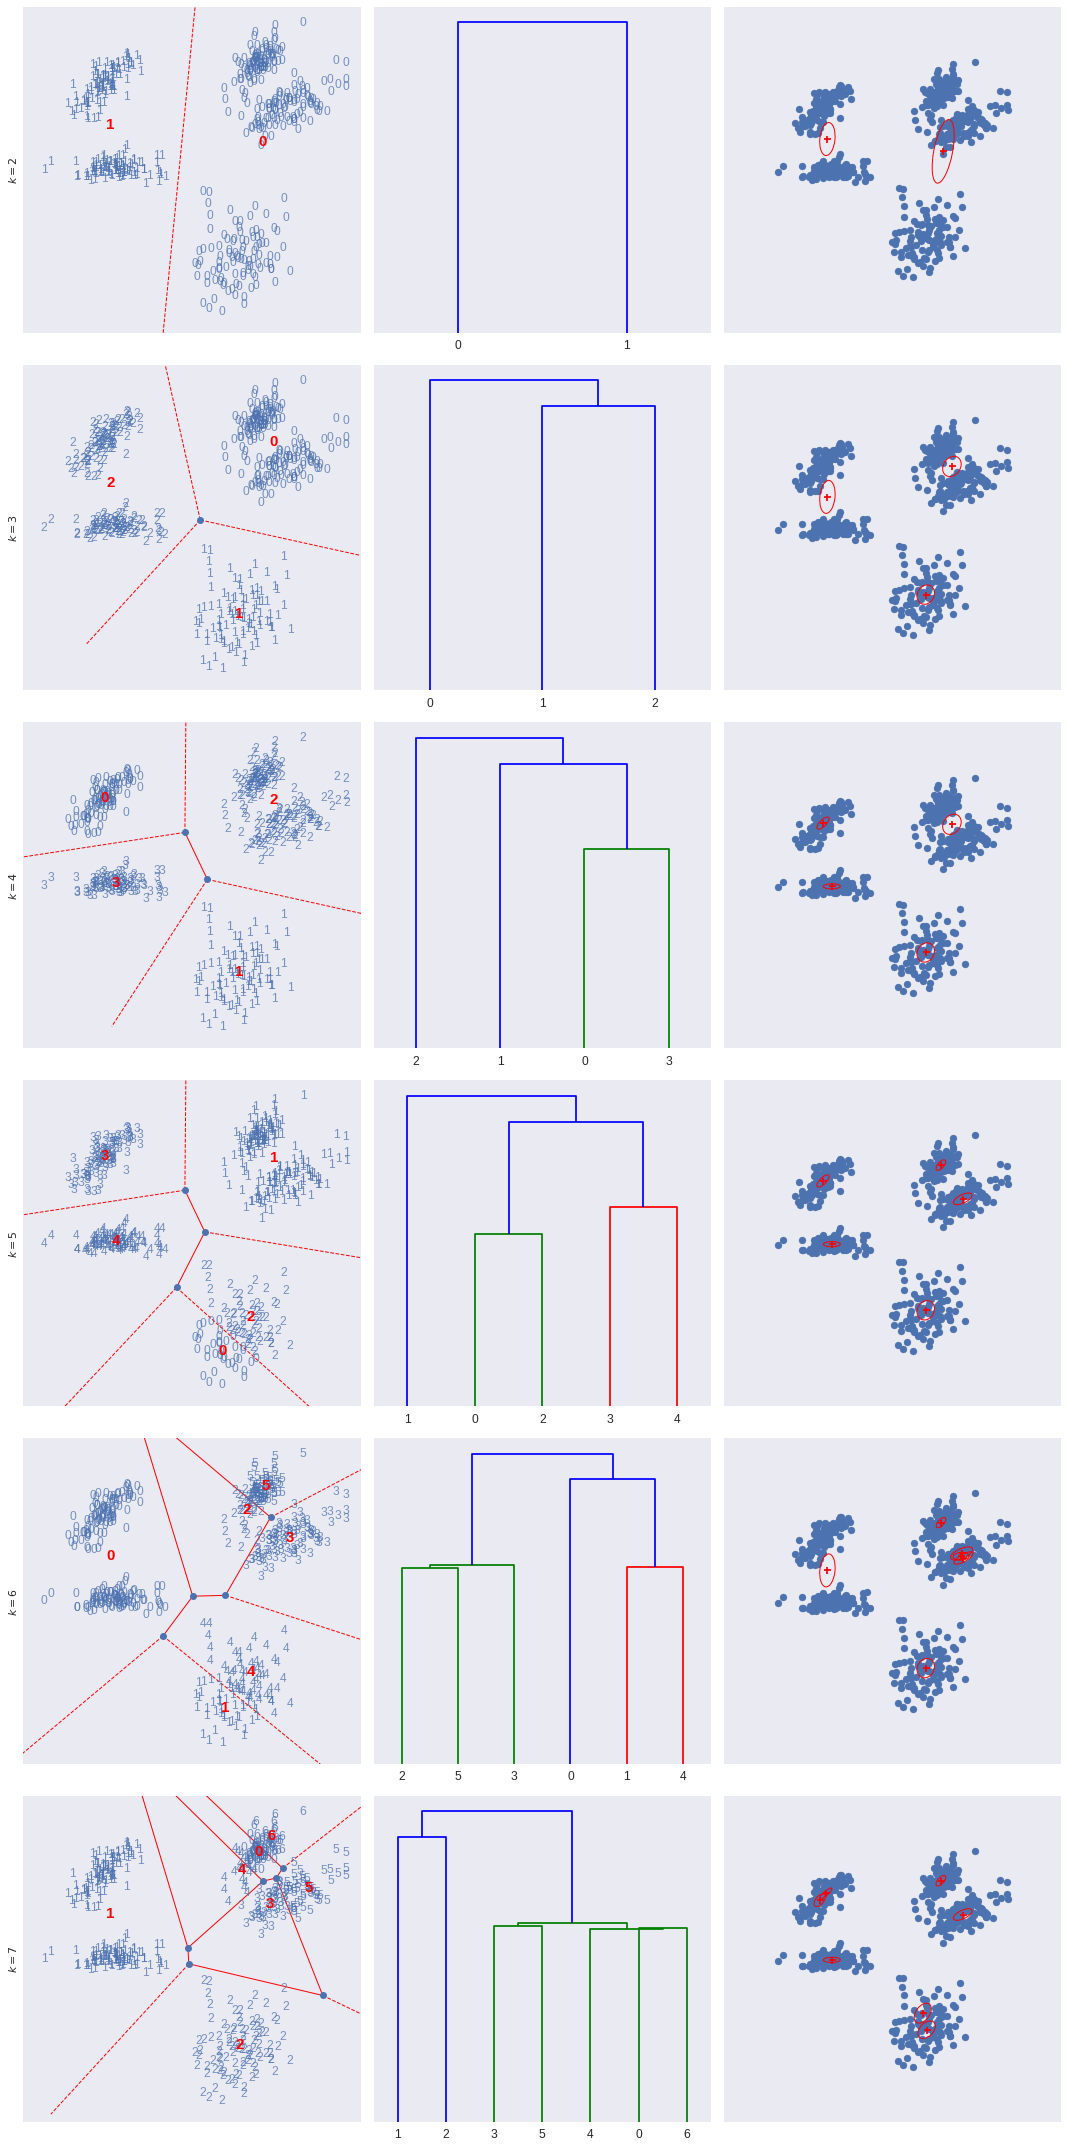
\includegraphics[scale=0.23]{../images/assignment7_local_optima.png}
    \caption{\small{5Gaussians - K-Means vs GMM - Local Optimum.
        \\ Rows show the different values of $k$.
        \\The first column is the result of K-Means clustering. The numbers indicate the centroid's indexes; each blue number is a data point, and each red number is a centroid. Red lines show the cluster's borders.
         \\The second column shows the result of the agglomeration on the K-Means' clusters, with the cluster's indexes on the x-axis.
         \\The third column is the GMM result. Red xs show the Gaussian's $\mu$s and red ellipses show the Gaussian's $\Sigma$s.}}
    \label{fig:assignment7_1}
\end{figure}

\subsection*{2.}

Given the random initialization of both algorithms, it could happen that the method defined in previous paragraph never finds a global optimum. However, given enough repetitions, this seems unlikely.

\subsection*{3.}

\Figref{assignment7_2,assignment7_3} show seemingly globally optimal solutions for $k=5$, with and without K-Means initialization in the GMM case.
\Tabref{assignment7_1,assignment7_2} show number of iterations taken by the two methods for different values of $k$, together with the K-Means loss value and GMM Log Likelihood.

\begin{figure}
    \centering
    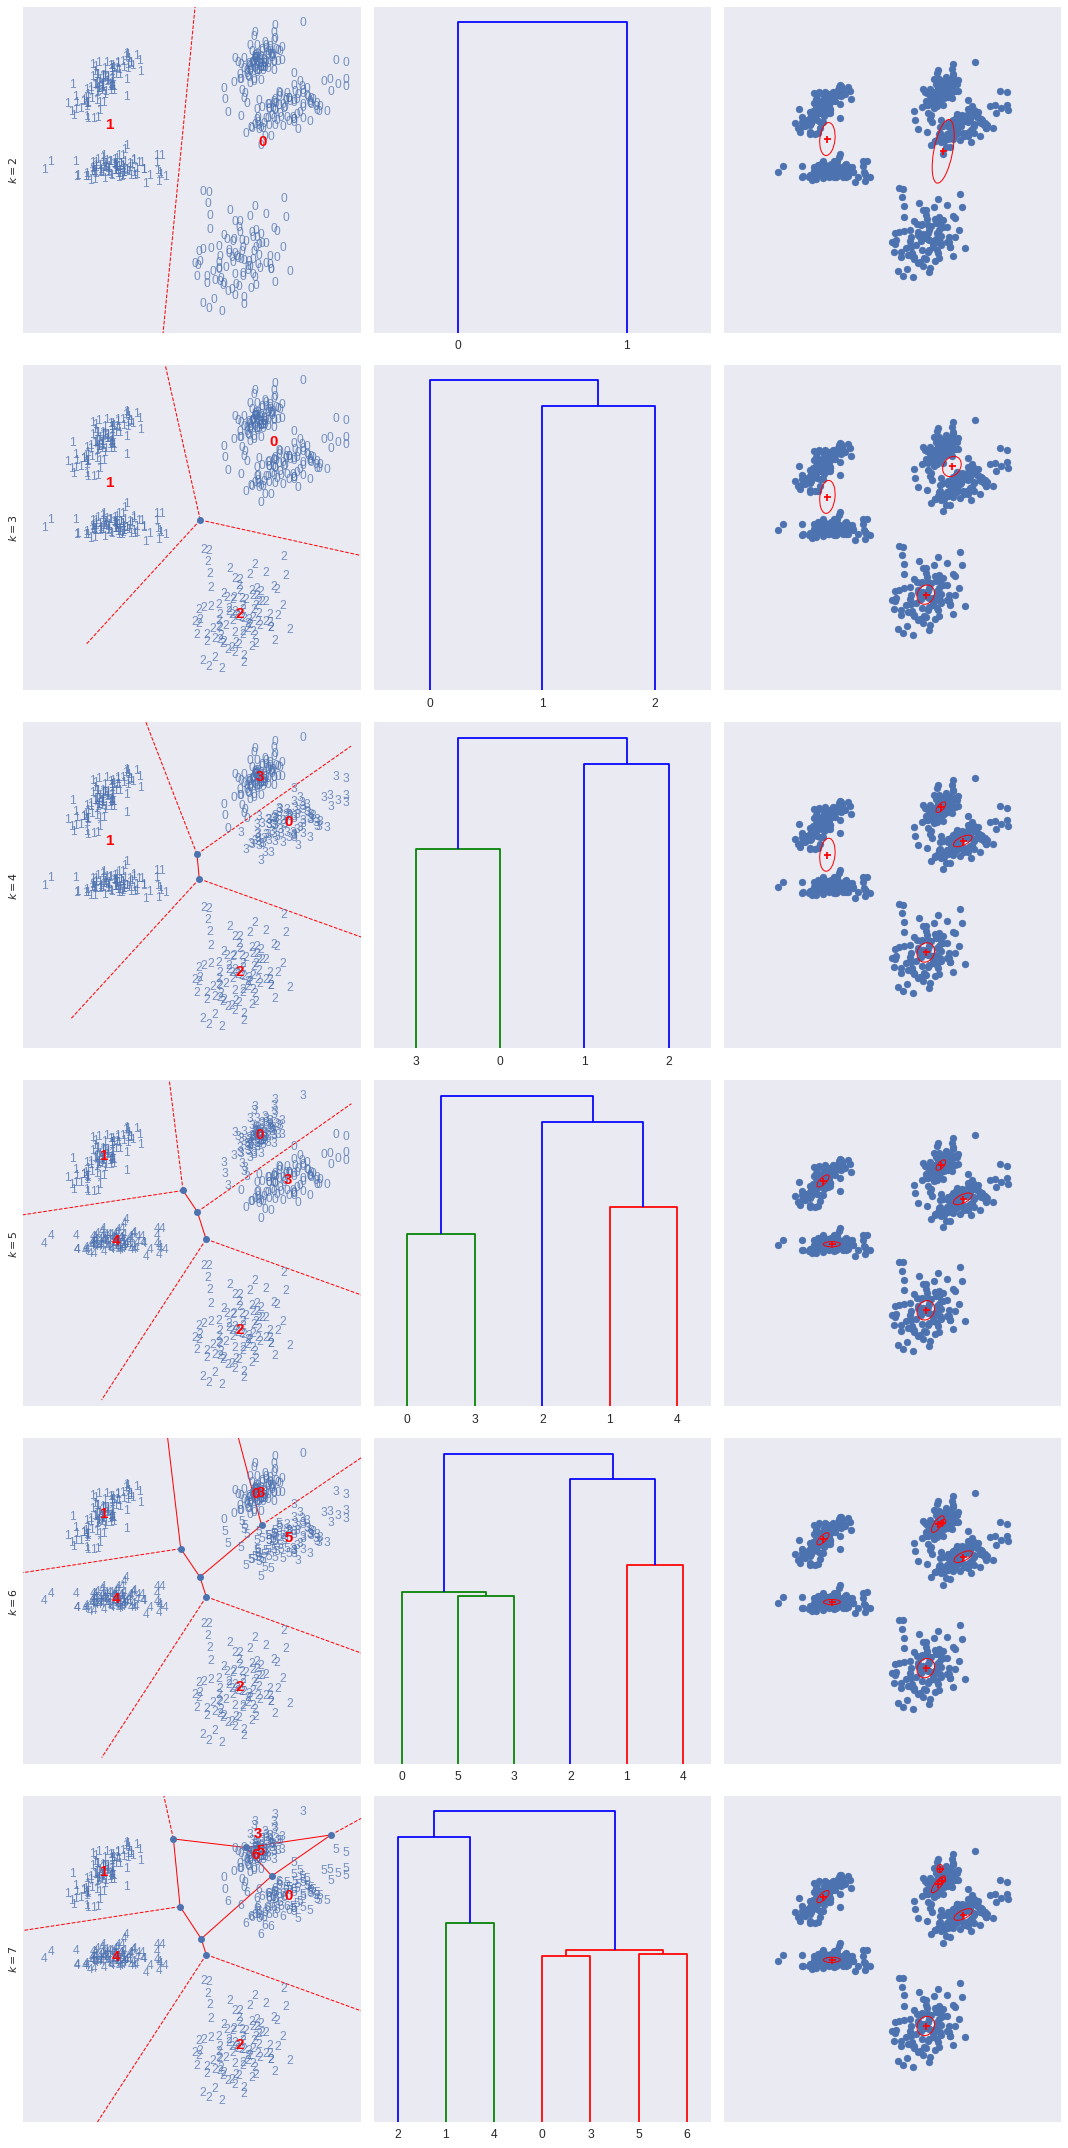
\includegraphics[scale=0.23]{../images/assignment7_kmeans_init.png}
    \caption{\small{5Gaussians - K-Means vs GMM (with K-Means initialization) - Global Optimum.
            \\ Rows show the different values of $k$.
            \\The first column is the result of K-Means clustering. The numbers indicate the centroid's indexes; each blue number is a data point, and each red number is a centroid. Red lines show the cluster's borders.
            \\The second column shows the result of the agglomeration on the K-Means' clusters, with the cluster's indexes on the x-axis.
            \\The third column is the GMM result. Red xs show the Gaussian's $\mu$s and red ellipses show the Gaussian's $\Sigma$s.}}
    \label{fig:assignment7_2}
\end{figure}

\begin{figure}
    \centering
    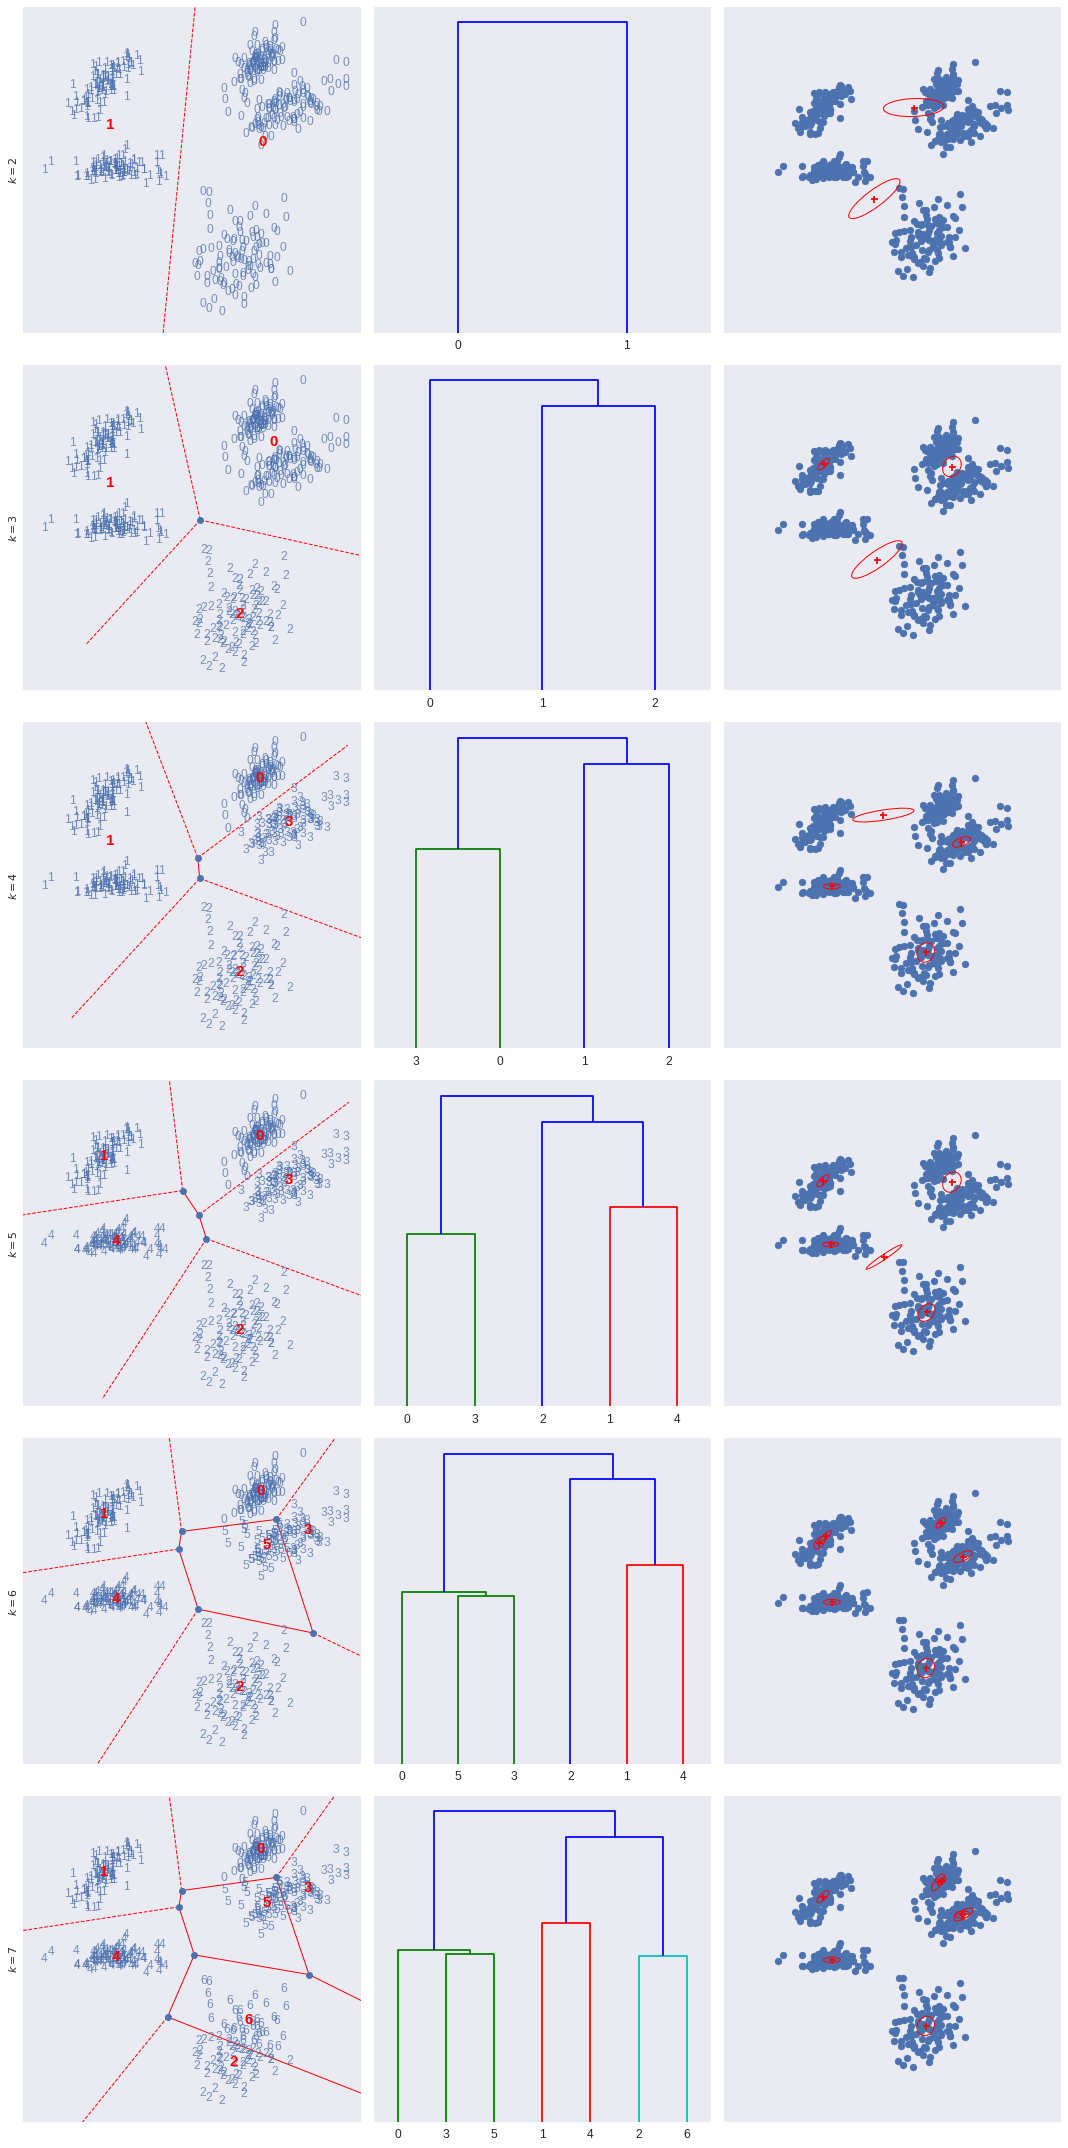
\includegraphics[scale=0.23]{../images/assignment7_no_kmeans_init.png}
    \caption{\small{5Gaussians - K-Means vs GMM (without K-Means initialization) - Global Optimum.
            \\ Rows show the different values of $k$.
            \\The first column is the result of K-Means clustering. The numbers indicate the centroid's indexes; each blue number is a data point, and each red number is a centroid. Red lines show the cluster's borders.
            \\The second column shows the result of the agglomeration on the K-Means' clusters, with the cluster's indexes on the x-axis.
            \\The third column is the GMM result. Red xs show the Gaussian's $\mu$s and red ellipses show the Gaussian's $\Sigma$s.}}
    \label{fig:assignment7_3}
\end{figure}

\begin{table}
    \centering
    \begin{tabularx}{\textwidth}{X|X|X|X|X}
        $k$ & Algo & Iterations & KM Loss & GMM Log-L \\
        \hline
        2   & KM   & 5          & 31.2617      & - \\
        2   & GMM  & 6          & -            & 10.4047 \\
        
        3   & KM   & 4          & 21.278       & - \\
        3   & GMM  & 5          & -            & 10.7997 \\
        
        4   & KM   & 7          & 20.9086      & - \\
        4   & GMM  & 25         & -            & 11.1441 \\
        
        5   & KM   & 10         & 18.0001      & - \\
        5   & GMM  & 25         & -            & 11.5501 \\
        
        6   & KM   & 14         & 18.428       & - \\
        6   & GMM  & 25         & -            & 11.5526 \\
        
        7   & KM   & 11         & 18.1382      & - \\
        7   & GMM  & 31         & -            & 11.5628
    \end{tabularx}
    \caption{\small{5Gaussians - K-Means vs GMM (with K-Means initialization) - Global Optimum.}}
    \label{tab:assignment7_1}
\end{table}

\begin{table}
    \centering
    \begin{tabularx}{\textwidth}{X|X|X|X|X}
        $K$ & Algo & Iterations & KM Loss & GMM Log-L \\
        \hline
        2   & KM   & 6          & 31.2611      & - \\
        2   & GMM  & 12         & -            & 10.1342 \\
        
        3   & KM   & 6          & 21.278       & - \\
        3   & GMM  & 16         & -            & 10.7797 \\
        
        4   & KM   & 6          & 18.3694      & - \\
        4   & GMM  & 21         & -            & 11.3226 \\
        
        5   & KM   & 7          & 18.0001      & - \\
        5   & GMM  & 28         & -            & 11.1467 \\
        
        6   & KM   & 12         & 17.7777      & - \\
        6   & GMM  & 46         & -            & 11.3509 \\
        
        7   & KM   & 5          & 18.2454      & - \\
        7   & GMM  & 26         & -            & 11.5994
    \end{tabularx}
    \caption{\small{5Gaussians - K-Means vs GMM (without K-Means initialization) - Global Optimum.}}
    \label{tab:assignment7_2}
\end{table}

\subsection*{4.}

\Figref{assignment7_1,assignment7_2,assignment7_3} all show the dendograms in their middle columns.
For $k=7$ and $k=6$, there are agglomerations that provide a very small reduction in the loss value, represented by the branch's height.
This means that the clusters being joined are close together, indicating that they are in reality a single cluster split in two because $k$ is too large.
Therefore, one policy could be to choose the largest $k$, such that the dendogram of the resulting clustering does not present such small reductions. In the case of the \verb|5gaussians| dataset that would be $k=5$.

\section*{Assignment 8.}
\subsection*{1.}

\Figref{assignment8} shows the results of multiple runs of both K-Means and GMM on the \verb|2gaussians| dataset.
Whereas K-Meas seems to always find similar local optima, GMM occasionally finds some good solutions (last two rows of \figref{assignment8_2}).


\begin{figure}
    \centering
    \begin{subfigure}[b]{0.45\textwidth}
        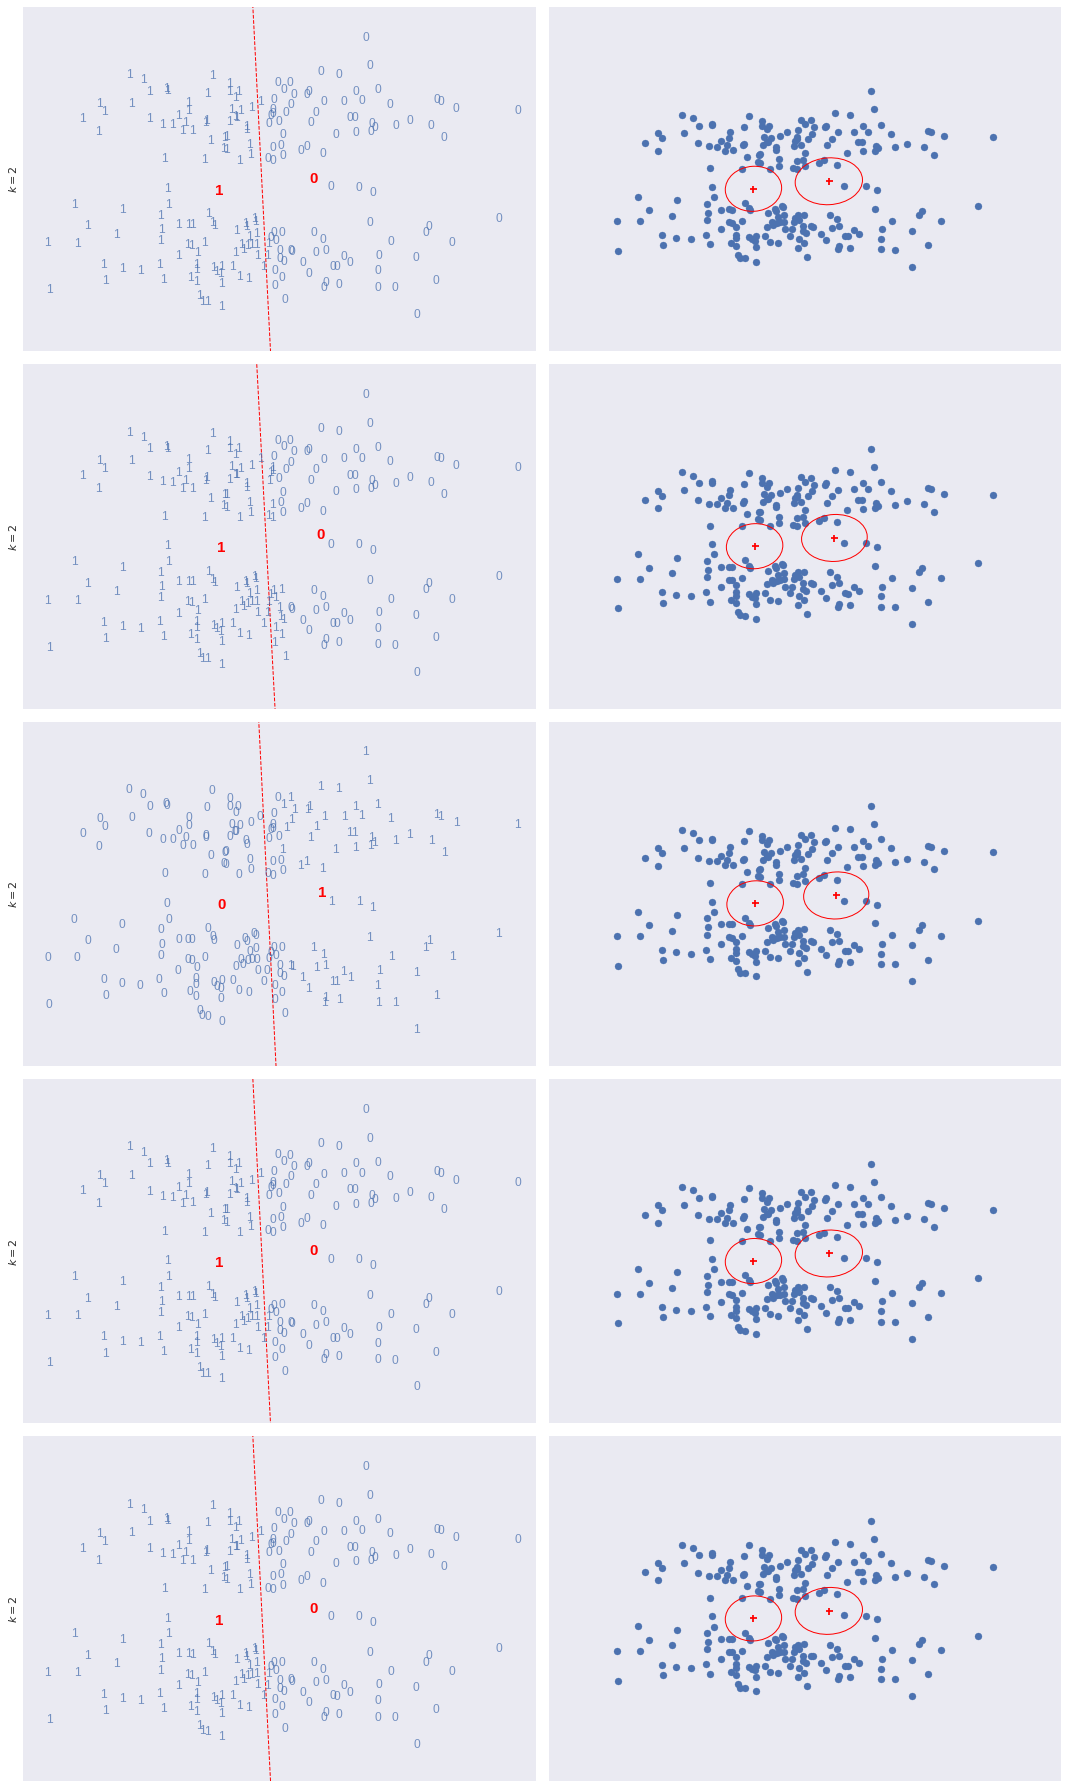
\includegraphics[scale=0.15]{../images/assignment8_kmeans_init.png}
        \caption{\small{With K-Means initialization.
                \\ GMM seems stuck in the same local optima as K-Means.}}
        \label{fig:assignment8_1}
    \end{subfigure}
    \hfill
    \begin{subfigure}[b]{0.45\textwidth}
        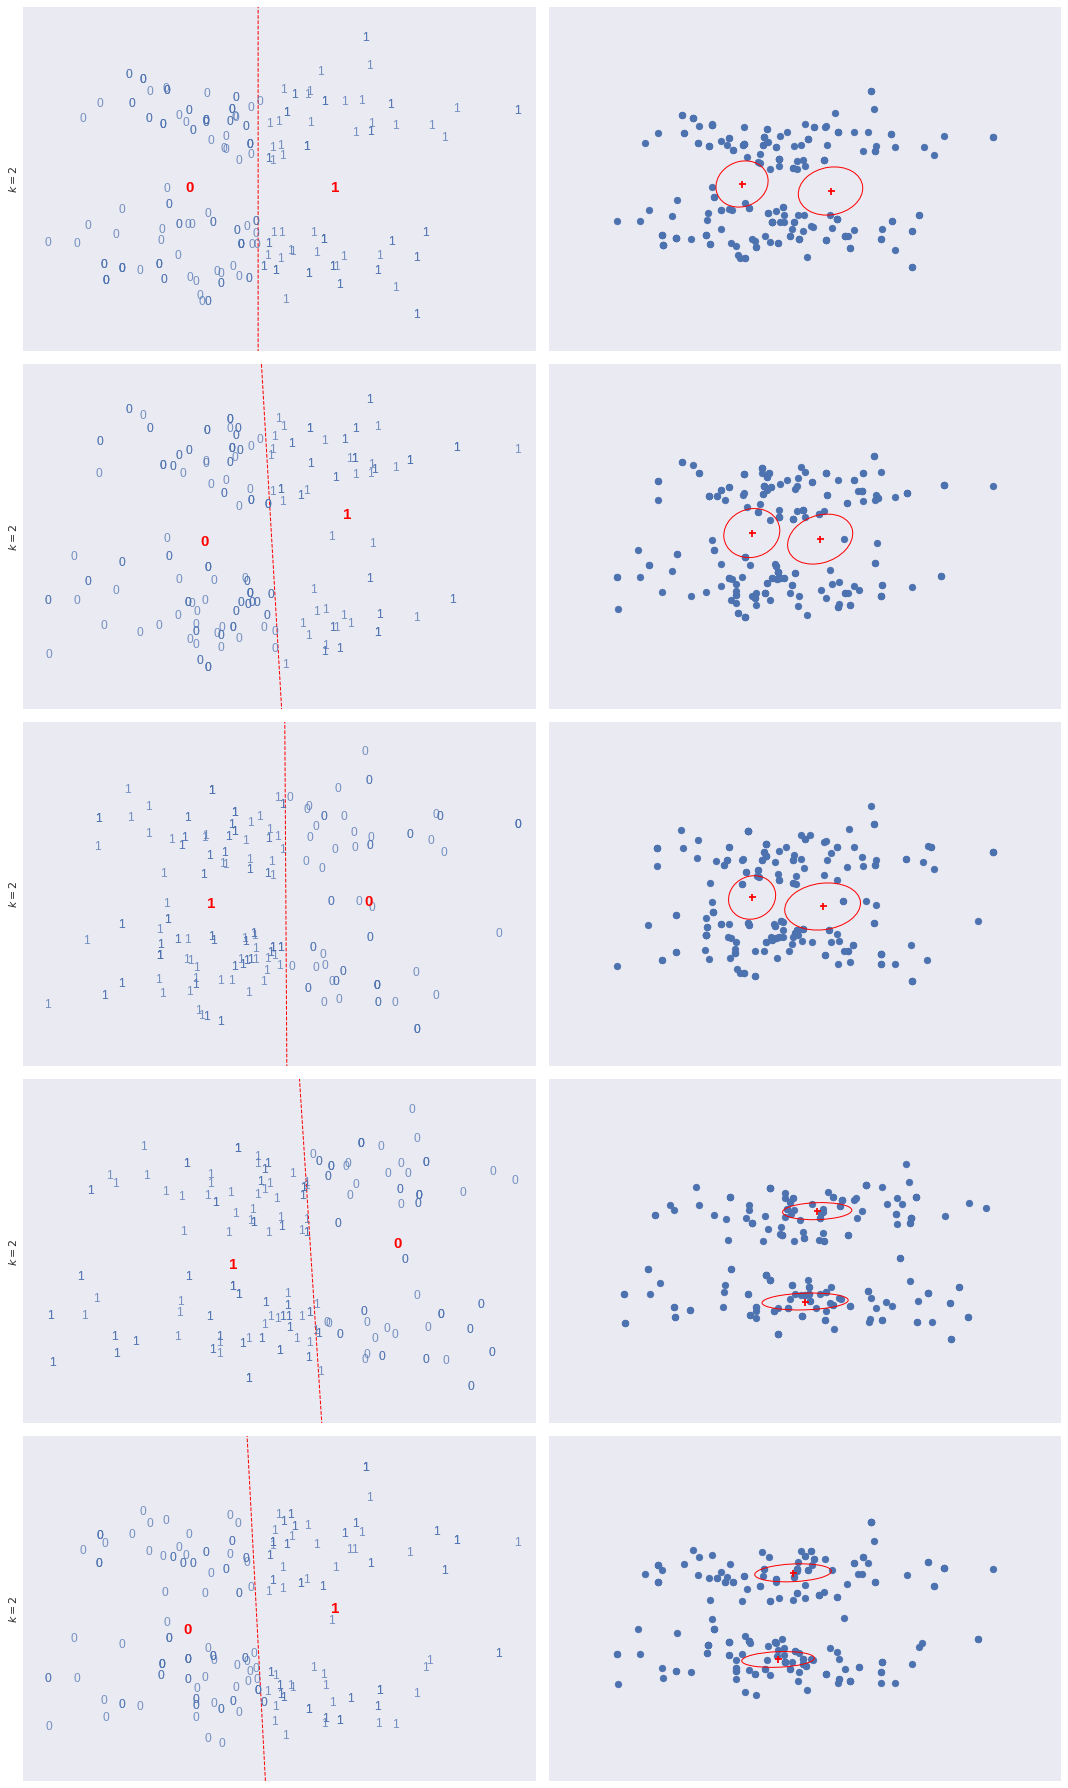
\includegraphics[scale=0.15]{../images/assignment8_no_kmeans_init.png}
        \caption{\small{Without K-Means initialization.
                \\ In some cases, GMM produces better results.}}
        \label{fig:assignment8_2}
    \end{subfigure}
        \caption{\small{2Gaussians - K-Means vs GMM.
                \\ Rows show the different runs of the algorithms.
                \\The first column is the result of K-Means clustering. The numbers indicate the centroid's indexes; each blue number is a data point, and each red number is a centroid. Red lines show the cluster's borders.
                \\The second column is the GMM result. Red xs show the Gaussian's $\mu$s and red ellipses show the Gaussian's $\Sigma$s.}}
    \label{fig:assignment8}
\end{figure}

\subsection*{2.}

Comparing the results in \figref{assignment8_1} against those in \figref{assignment8_2}, and also the different runs in \figref{assignment8_2}, one could conclude that GMM depends heavily on a good initialization to deliver good clusters.

\section*{Assignment 9.}
\subsection*{1.}

\Figref{assignment9_1} and \tabref{assignment9} show the comparison between the two methods on the \verb|usps| dataset. In the case of K-Means, the label predicted was the most common label among the points assigned to each cluster (see \verb|sheet2.py|, function \verb|km_cluster_idx|, line 350). In the case of GMM, first the most likely cluster assignment for each point was calculated, and then the same procedure as for K-Means was performed (see \verb|sheet2.py|, function \verb|gmm_cluster_idx|, line 362).

From the tables, it seems that K-Means outperformed GMM in this task. It is unclear whether it is because GMM only reached a local optima, or because some intrinsic characteristic of the method. It should be noted that several runs of both K-Means and GMM were performed with similar results (not in the report due to space considerations).

\begin{figure}
    \centering
    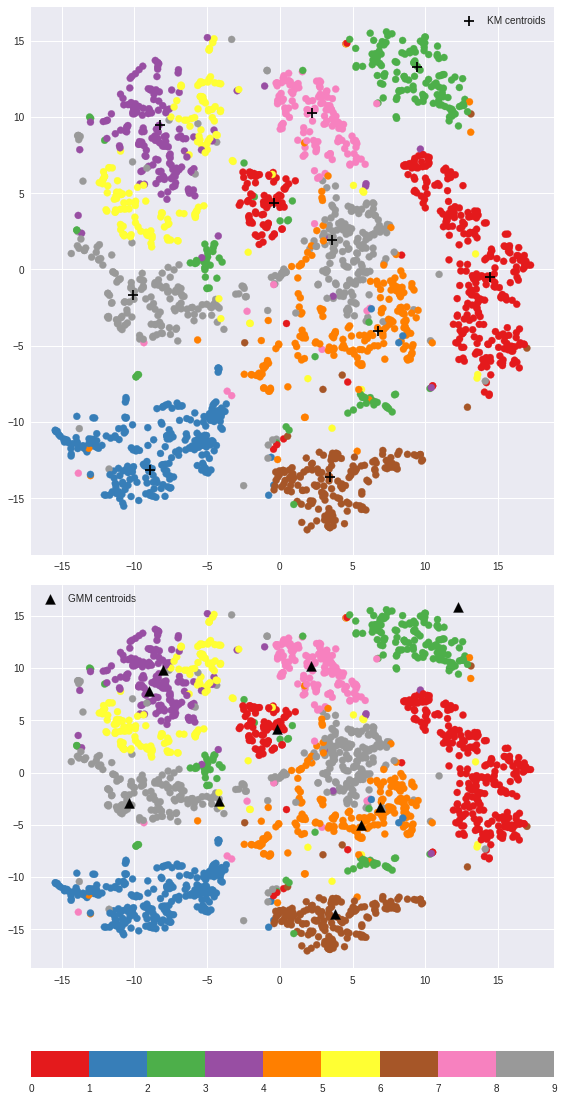
\includegraphics[scale=0.5]{../images/assignment9_2.png}
    \caption{\small{USPS - K-Means vs GMM - Centroid comparison.
             \\ t-SNE projection of the data in 2D, with the K-Means centroids (above, black crosses) and GMM centroids (below, black triangles) superimposed.}}
    \label{fig:assignment9_1}
\end{figure}



\begin{table}
    \centering
    \begin{subtable}[b]{\textwidth}
        \centering
        \begin{tabularx}{\textwidth}{X|X|X|X|X}
            class        & precision & recall & f1-score & support \\
            \hline
            0           & 0.86      & 0.81   & 0.84     & 359 \\
            1           & 0.92      & 0.97   & 0.95     & 264 \\
            2           & 0.93      & 0.64   & 0.76     & 198 \\
            3           & 0.49      & 0.74   & 0.59     & 166 \\
            4           & 0.64      & 0.57   & 0.60     & 200 \\
            5           & 0.00      & 0.00   & 0.00     & 160 \\
            6           & 0.61      & 0.81   & 0.70     & 170 \\
            7           & 0.78      & 0.76   & 0.77     & 147 \\
            8           & 0.54      & 0.55   & 0.55     & 166 \\
            9           & 0.39      & 0.63   & 0.48     & 177 \\
            \hline
            avg / total & 0.66      & 0.68   & 0.66     & 2007
        \end{tabularx}
        \caption{\small{K-Means report.}}
        \label{tab:assignment9_1}
    \end{subtable}
    \\
    \begin{subtable}[b]{\textwidth}
        \centering
        \begin{tabularx}{\textwidth}{X|X|X|X|X}
            class       & precision & recall & f1-score & support \\
            \hline
            0           & 0.63      & 0.97   &  0.76    & 359 \\
            1           & 0.41      & 0.99   &  0.58    & 264 \\
            2           & 0.96      & 0.67   &  0.79    & 198 \\
            3           & 0.66      & 0.49   &  0.57    & 166 \\
            4           & 0.69      & 0.72   &  0.71    & 200 \\
            5           & 0.58      & 0.50   &  0.54    & 160 \\
            6           & 0.00      & 0.00   &  0.00    & 170 \\
            7           & 0.72      & 0.75   &  0.74    & 147 \\
            8           & 0.61      & 0.19   &  0.29    & 166 \\
            9           & 0.00      & 0.00   &  0.00    & 177 \\
            \hline
            avg / total & 0.53      & 0.59   &  0.53    & 2007
        \end{tabularx}
        \caption{\small{GMM report.}}
        \label{tab:assignment9_2}
    \end{subtable}
    \caption{\small{USPS - K-Means vs GMM classification report}}
    \label{tab:assignment9}
\end{table}

\subsection*{2.}

\Figref{assignment9_2} shows the required plots.

\begin{figure}
    \centering
    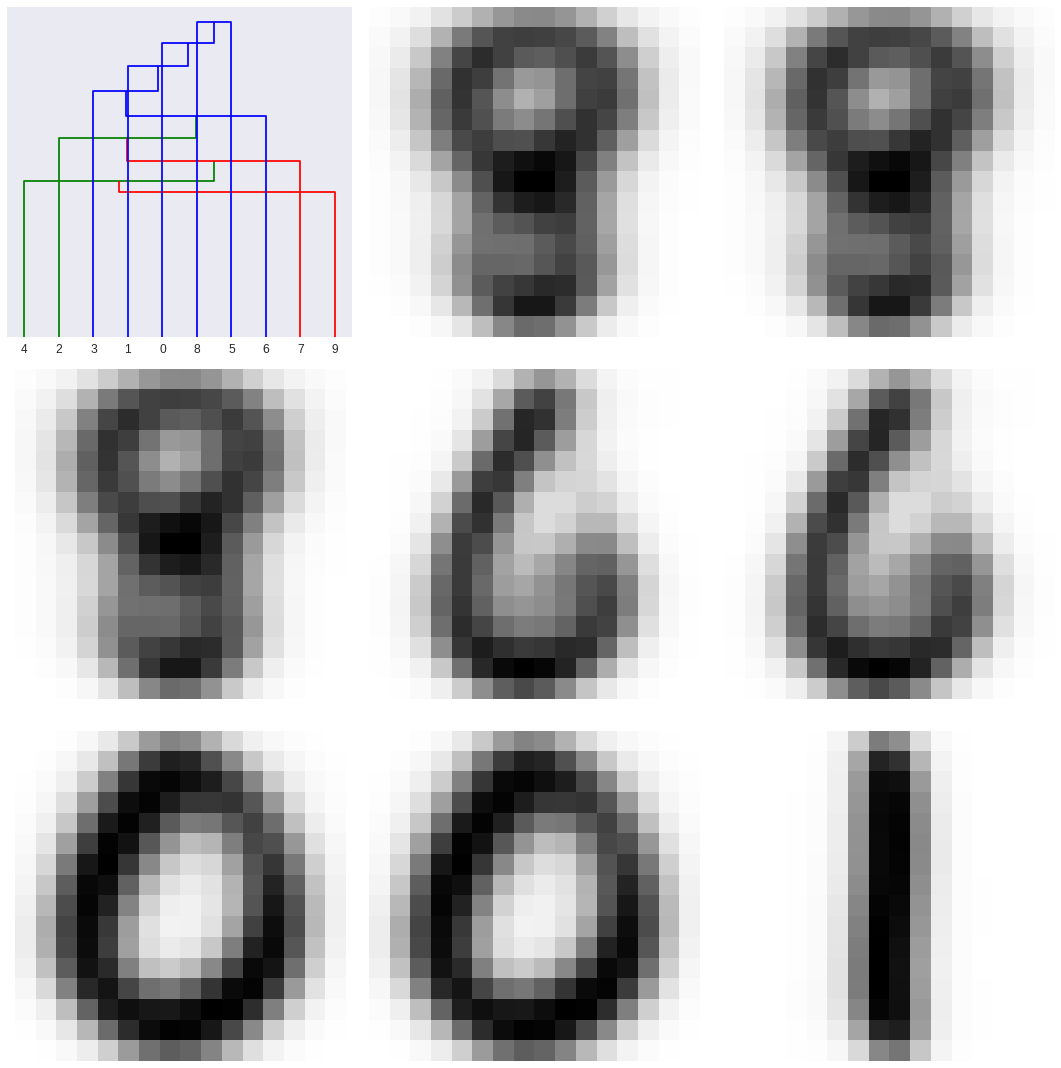
\includegraphics[scale=0.35]{../images/assignment9_1.png}
    \caption{\small{USPS - K-Means Dendogram (upper left corner) and centroids visualization (everything else, using \texttt{imshow}).}}
    \label{fig:assignment9_2}
\end{figure}

\section*{Assignment 10.}
\subsection*{2.}
A hundred runs of GMM with K-Means initialization and $k=3$ were run, always with the same results, shown in \tabref{assignment10}, with a final log likelihood of $10.539$.
\begin{table}
    \centering
    \begin{tabularx}{\textwidth}{X|XXX}
        cluster Nr &  vector     &            & \\
        \hline
        0          & -0.07117879 & 0.06915395 & -1.01893152 \\
        \hline
        1          &  0.11408639 & 0.14507352 & -0.15056507 \\
        \hline
        2          &  0.50019964 & 0.04448412 &  1.0177551 \\
        \hline
    \end{tabularx}
    \caption{\small{lab\_data - GMM $\protect\mu_k$ vectors.}}
    \label{tab:assignment10}
\end{table}
\subsection*{3.}

After computing \verb|gammaidx| with different values of $k$ (from \verb|1| to \verb|len(lab_data['X']) - 1|), both the \verb|auc| funciton from \verb|sheet1| and \verb|scikit-learn|'s \verb|roc_auc_score| function reported a best AUC score of $0.8766$ with $k=6$.

\subsection*{4.}
The "inlier score" was calculated as the log likelihood of a point given the GMM model (see \verb|sheet2.py|, funciton \verb|in_score|, line 474).

With this procedure an AUC score of $0.8745$, slightly below what was obtained with the \verb|gammaidx|.

\Figref{assignment10_1} shows the ROC curves for both methods.


\begin{figure}
    \centering
    \begin{subfigure}[b]{0.45\textwidth}
        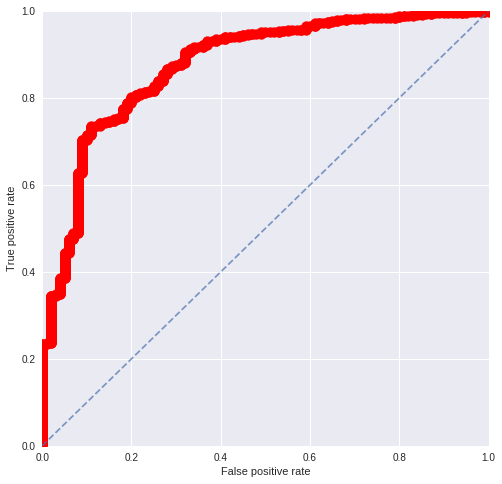
\includegraphics[scale=0.3]{../images/assignment10_3.png}
        \caption{\small{\texttt{gammaidx} with $\protect k=6$.}}
        \label{fig:assignment10_1_1}
    \end{subfigure}
    \hfill
    \begin{subfigure}[b]{0.45\textwidth}
        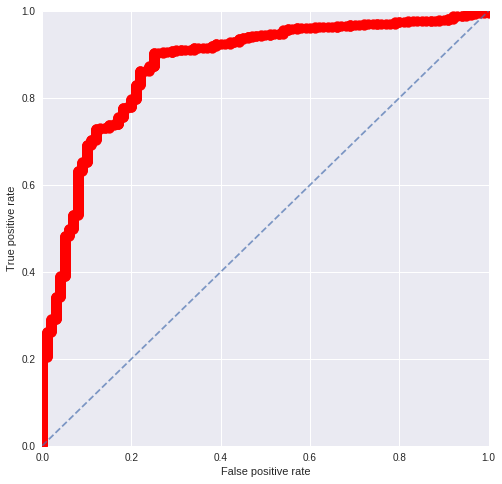
\includegraphics[scale=0.3]{../images/assignment10_4.png}
        \caption{\small{GMM with $\protect k=3$.}}
        \label{fig:assignment10_1_2}
    \end{subfigure}
    \caption{\small{lab\_data - ROC curves.}}
    \label{fig:assignment10_1}
\end{figure}

\end{document}

